\documentclass[a4paper]{article}
\usepackage[utf8]{inputenc}
\usepackage[spanish, es-tabla, es-noshorthands]{babel}
\usepackage[table,xcdraw]{xcolor}
\usepackage[a4paper, footnotesep=1.25cm, headheight=1.25cm, top=2.54cm, left=2.54cm, bottom=2.54cm, right=2.54cm]{geometry}
%\geometry{showframe}

%\usepackage{wrapfig}			%Wrap figure in text
\usepackage[export]{adjustbox}	%Move images
\usepackage{changepage}			%Move tables

\usepackage{tikz}
\usepackage{amsmath}
\usepackage{amsfonts}
\usepackage{amssymb}
\usepackage{float}
\usepackage{graphicx}
\usepackage{caption}
\usepackage{subcaption}
\usepackage{multicol}
\usepackage{multirow}
\usepackage{wrapfig}
\setlength{\doublerulesep}{\arrayrulewidth}
\usepackage{booktabs}
\usepackage[numbib, nottoc, notlot, notlof]{tocbibind}

\usepackage{hyperref}
\hypersetup{
    colorlinks=true,
    linkcolor=blue,
    filecolor=magenta,      
    urlcolor=blue,
    citecolor=blue,    
}

%Change Font Size

% #1 = size, #2 = text
\newcommand{\setparagraphsize}[2]{{\fontsize{#1}{6}\selectfont#2 \par}}		%Cambia el size de todo el parrafo
\newcommand{\setlinesize}[2]{{\fontsize{#1}{6}\selectfont#2}}				%Cambia el font de una oración

\newcommand{\note}[1]{
	\begin{center}
		\huge{ \textcolor{red}{#1} }
	\end{center}
}

%FONTS (IMPORTANTE): Compilar en XeLaTex o LuaLaTeX
\usepackage{anyfontsize}	%Font size
\usepackage{fontspec}		%Font type

\usepackage{etoolbox}
\usepackage{todonotes}

\newcommand{\observacion}[2]{  \ifnumequal{1}{#1}{ { \todo[inline,backgroundcolor=red!25,bordercolor=red!100]{\textbf{Observación: #2}} } }{  }  }

\setcounter{topnumber}{2}
\setcounter{bottomnumber}{2}
\setcounter{totalnumber}{4}
\renewcommand{\topfraction}{0.85}
\renewcommand{\bottomfraction}{0.85}
\renewcommand{\textfraction}{0.15}
\renewcommand{\floatpagefraction}{0.8}
\renewcommand{\textfraction}{0.1}
\setlength{\floatsep}{5pt plus 2pt minus 2pt}
\setlength{\textfloatsep}{5pt plus 2pt minus 2pt}
\setlength{\intextsep}{5pt plus 2pt minus 2pt}

\newcommand{\quotes}[1]{``#1''}
\usepackage{array}
\newcolumntype{C}[1]{>{\centering\let\newline\\\arraybackslash\hspace{0pt}}m{#1}}
\usepackage[american]{circuitikz}
\usetikzlibrary{calc}
\usepackage{fancyhdr}
\usepackage{units} 

\graphicspath{{../Control de posición no lineal/}{../Control de fuerza no lineal/}{../Control híbrido no lineal/}{../Referencias/}{../Deducción de modelo/}{../Conclusiones/}}

\pagestyle{fancy}
\fancyhf{}
\lhead{22.99 - Automación Industrial}
\rhead{Lambertucci, Londero B., Maselli, Mechoulam}
\rfoot{Página \thepage}

%Items con bullets y no cuadrados
\renewcommand{\labelitemi}{\textbullet }


\begin{document}

\def\verObs{0}

%%%%%%%%%%%%%%%%%%%%%%%%%
%		Caratula		%
%%%%%%%%%%%%%%%%%%%%%%%%%

\setmainfont{AvenirLTStd-Roman}[Path = ./Utils/, Extension = .otf]

\begin{titlepage}

\begin{tikzpicture}[remember picture, overlay, black, line width = 0.5pt]
	\coordinate (a) at (-2cm,2cm);
	\coordinate (b) at (17cm,-25.5cm);
	
	\coordinate (ap) at (-2.1cm,2.1cm);
	\coordinate (bp) at (17.1cm,-25.6cm);
	
	\draw[] (a) -| (b);
	\draw[] (a) |- (b);
	
	\draw[] (ap) -| (bp);
	\draw[] (ap) |- (bp);
	
	%footnotesep=1.25cm, headheight=1.25cm, top=2.54cm, left=2.54cm, bottom=2.54cm, right=2.54cm

\end{tikzpicture}

\begin{figure}[H]
	
\includegraphics[width=0.3\linewidth, right]{./Utils/ITBA_1}
\end{figure}

\vspace*{1.5cm}

\noindent \textbf{\setlinesize{12}{INSTITUTO TECNOLÓGICO DE BUENOS AIRES - ITBA}}

\noindent \textbf{\setlinesize{12}{ESCUELA DE INGENIERÍA Y TECNOLOGÍA}}

\vspace*{4cm}

\begin{center}
	\setlinesize{24}{ \textbf{TRABAJO PRÁCTICO FINAL} }
	
	\vspace*{1.5cm}
	%\setlinesize{24}{ \textbf{Subtítulo del trabajo (cuando corresponda)} }
	\vspace*{1.0cm}
\end{center}
\begin{center}
	\setlinesize{18}{ \textbf{MANUAL DE USUARIO} }
	
	\vspace*{1.5cm}
	%\setlinesize{24}{ \textbf{Subtítulo del trabajo (cuando corresponda)} }
	\vspace*{1.0cm}
\end{center}
\begin{figure}[H]
\begin{adjustwidth}{-1cm}{}
\begin{tabular}{llr} 
	\textbf{AUTORES:}
	& \textbf{Lambertucci, Guido Enrique} & \textbf{(Leg. N}$\mathbf{^o}$ \textbf{58009)} \\
	& \textbf{Londero Bonaparte, Tomás Guillermo} & \textbf{(Leg. N}$\mathbf{^o}$ \textbf{58150)} \\
	& \textbf{Mechoulam, Alan}  &  \textbf{(Leg. N}$\mathbf{^o}$ \textbf{58438)}\\
	& \textbf{Maselli, Carlos Javier} &  \textbf{(Leg. N}$\mathbf{^o}$ \textbf{59564)} \\
	 
 &  & \\
 &  & \\
	\textbf{DOCENTES}:
	& \textbf{Arias, Rodolfo Enrique} & \\
	& \textbf{Sofio Avogadro, Federico} & \\
	& \textbf{Spinelli, Mariano Tomás} & \\
\end{tabular}
\end{adjustwidth}
\end{figure}

\vspace*{0.5cm}
\center{
%{\noindent \setparagraphsize{12}{\textbf{TRABAJO PRÁCTICO N$^{\circ}$1}}}
{\noindent \setparagraphsize{12}{\textbf{\textsc{22.90 - Automación Industrial}}}}
}
\vspace*{1.5cm}

\center{\textbf{BUENOS AIRES}}

\end{titlepage}


\setmainfont{calibri-regular}[Path = ./Utils/, Extension = .ttf, BoldFont=calibrib, ItalicFont=calibrii, BoldItalicFont=calibriz]

%%%%%%%%%%%%%%%%%%%%%
%		Informe		%
%%%%%%%%%%%%%%%%%%%%%

\Section{Introducción}
En este breve informe se explica como poder correr el código del trabajo y como utilizarlo.

\Section{Dependencias}
Las dependencias necesarias son:
\begin{itemize}
\item \href{https://petercorke.com/toolboxes/robotics-toolbox/}{Peter Corke Robotics Toolbox}
\item \href{https://petercorke.com/toolboxes/machine-vision-toolbox/}{Peter Corke Vision Toolbox}
\item \href{https://la.mathworks.com/products/matlab.html}{Matlab 2018}
\end{itemize}

\Section{Correr el trabajo}
Para poder utilizar la interfaz gráfica se debe abrir la carpeta \quotes{Widow} y correr el archivo llamado \quotes{main.m} en Matlab 2018. Así se abrirá la siguiente interfaz:
\begin{figure}[H]
	\centering
	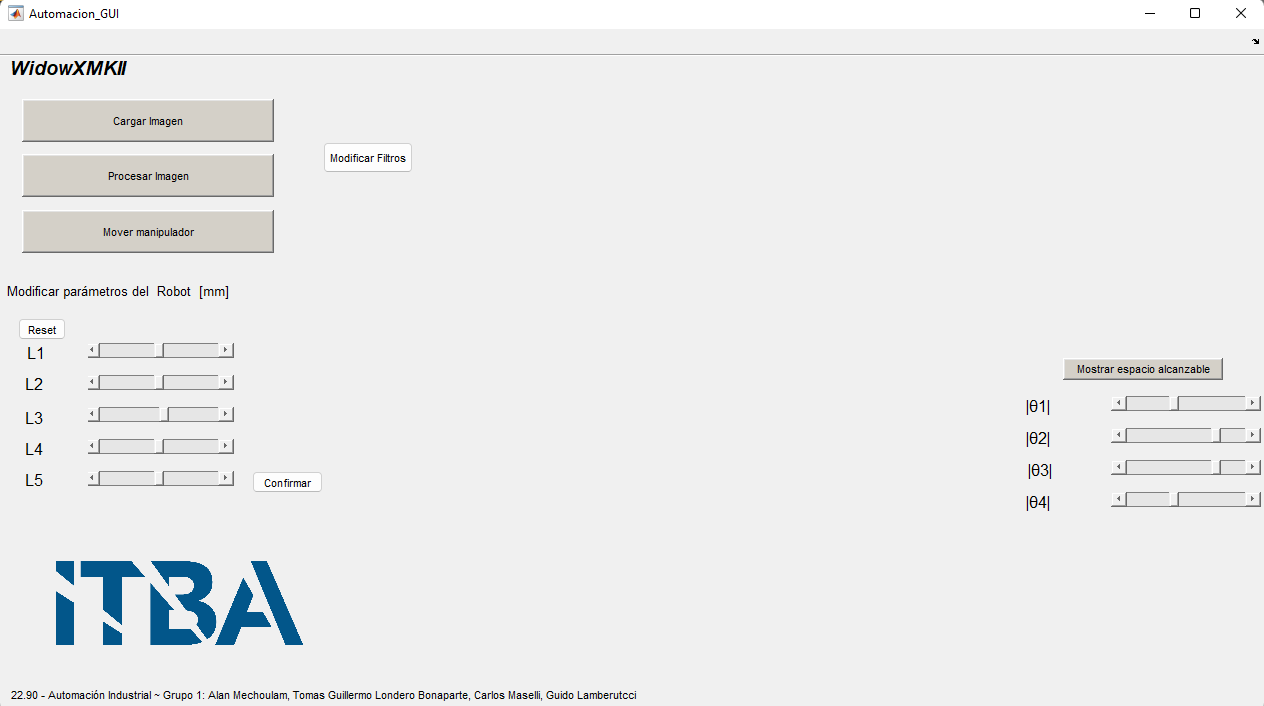
\includegraphics[width=\linewidth]{GUI}
	\caption{GUI.}	
	\label{fig:GUI}
\end{figure}

\Section{Utilización}

\Subsection{Flujo de uso}

Lo primero a hacer es cargar una imagen. Se debe presionar el botón \quotes{Cargar Imagen} y elegir una que cumpla con el formato de la presentada en la consigna. Al hacer esto se verá la siguiente pantalla:
\begin{figure}[H]
	\centering
	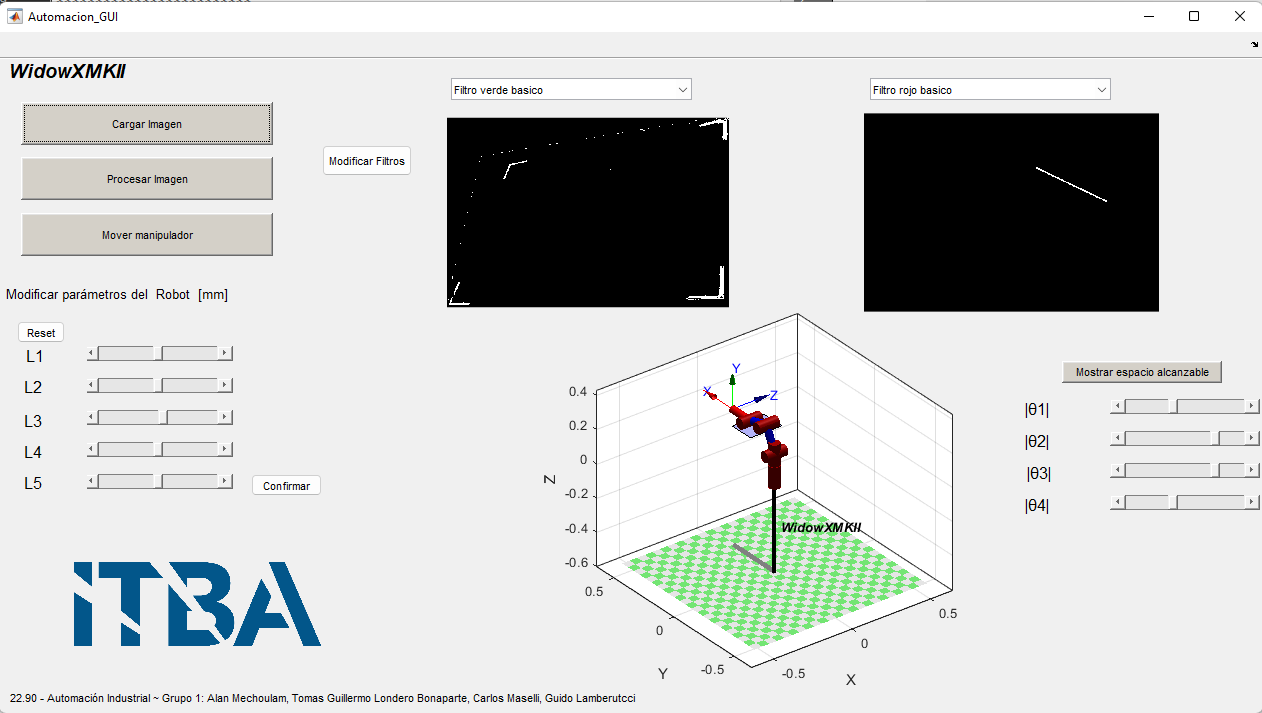
\includegraphics[width=\linewidth]{init}
	\caption{Inicialización.}	
	\label{fig:Inicializacion}
\end{figure}

Al cargarla imagen se hace un filtrado básico de los colores y se muestra el manipulador. 
Una vez hecho esto, se accede a las opciones de \quotes{Mostrar espacio alcanzable} y \quotes{Modificar manipulador}.

Se brinda la posibilidad de cambiar en los marcos presentes los distintos tipos de filtros que y figuras que se usan a lo largo del proceso. Esto se puede cambiar desde los \quotes{Drop Down Menus} que se encuentran por encima de cada imagen.

Si se desea continuar, se debe presionar el botón de \quotes{Procesar Imagen}. Al hacer esto se realiza el filtrado, quitando todo el ruido posible y obteniendo tantos las coordenadas de las esquinas como las de la linea.

Además se brinda acceso a un menú con todos los pasos intermedios en el filtrado.
\begin{figure}[H]
	\centering
	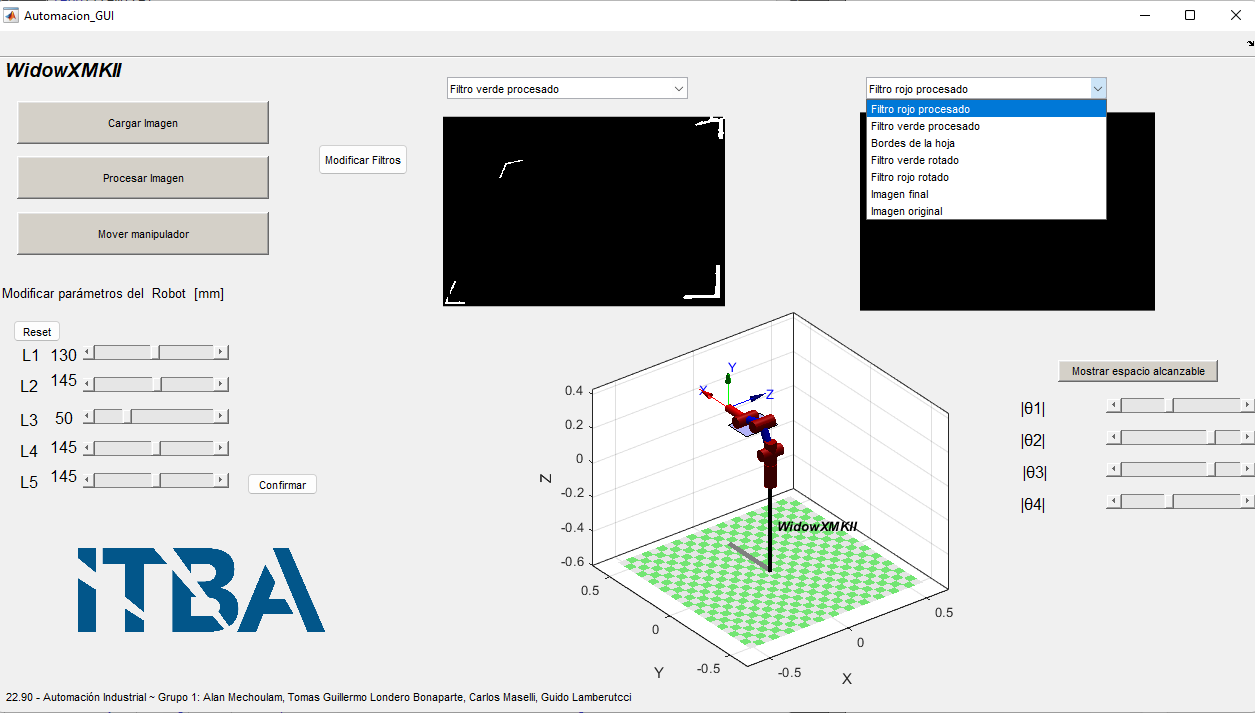
\includegraphics[width=\linewidth]{ddm}
	\caption{Imagen procesada y opciones.}	
	\label{fig:ddm}
\end{figure}

Luego, al utilizar el botón \quotes{Mover manipulador}, se logra que el robot recree el movimiento, como se ve en la mesa dibujada en pantalla.
\begin{figure}[H]
	\centering
	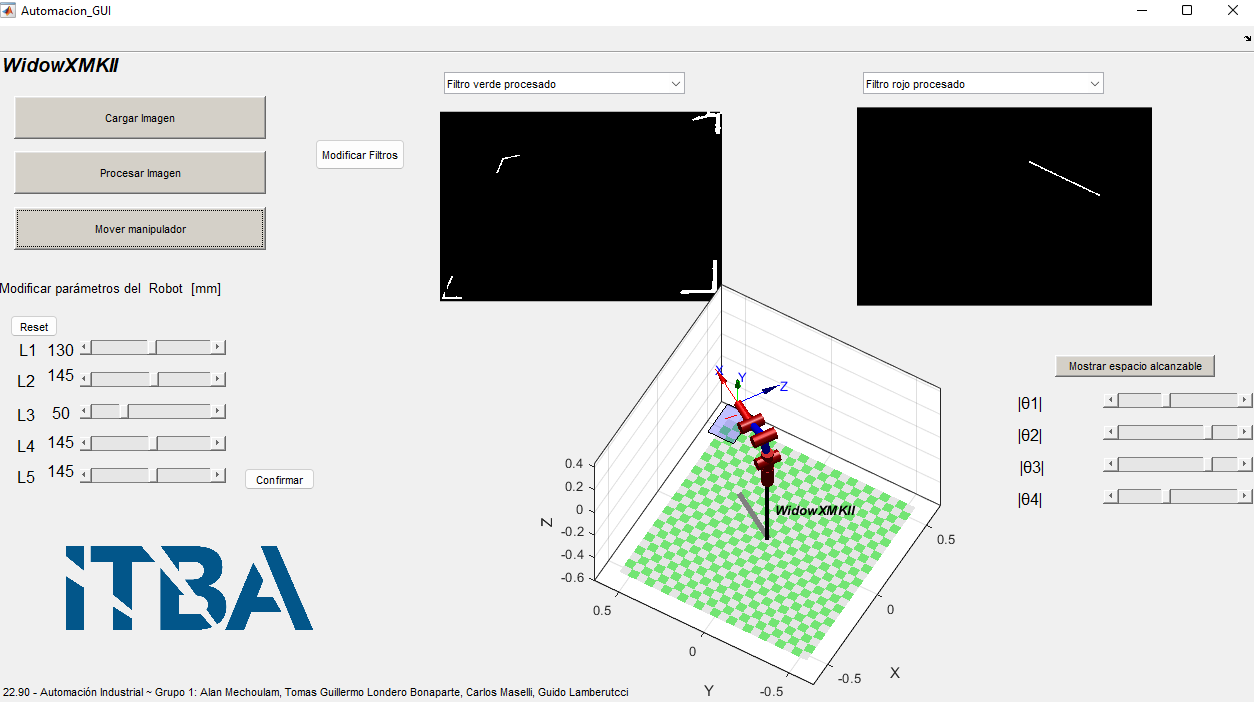
\includegraphics[width=\linewidth]{linea}
	\caption{Manipulador una vez dibujado.}	
	\label{fig:linea}
\end{figure}

Si se quisiera se puede cargar una nueva imagen y repetir el proceso.

\Subsection{Configuración de longitudes}

Es posible configurar las longitudes del manipulador durante la ejecución al cambiar los valores en la GUI.
\begin{figure}[H]
	\centering
	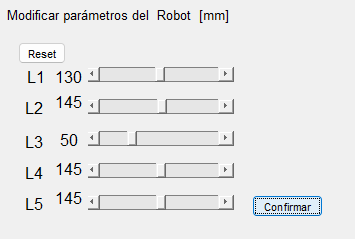
\includegraphics[width=0.35\linewidth]{mm}
	\caption{Modificación de parámetros.}	
	\label{fig:mm}
\end{figure}

Esta modificación es para valores dentro de un desvío del 10\% del nominal para cada dimensión del manipulador.

Al tocar en \quotes{Confirmar} se guardan los valores ingresados mediante el slider.
Para volver a valores por defecto se debe tocar el botón \quotes{Reset}.

\Subsection{Visualización de espacio alcanzable}

Para visualizar el espacio alcanzable del manipulador, basta con presionar el botón \quotes{Mostrar espacio alcanzable}. Los ángulos de libertad que tienen los joints son configurables. Es importante mencionar que la variación de dicho parámetro es en módulo.
\begin{figure}[H]
	\centering
	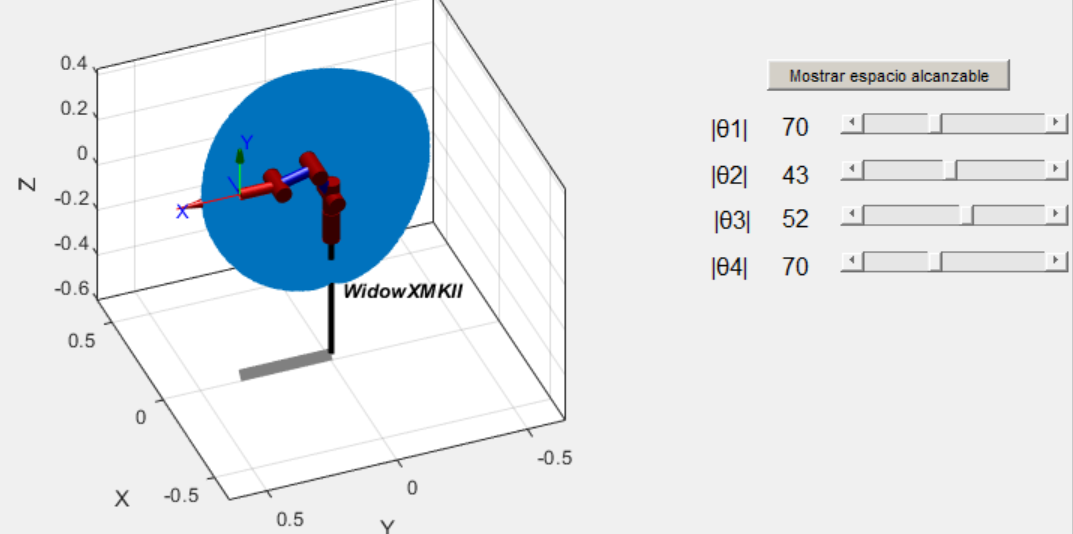
\includegraphics[width=0.7\linewidth]{alcanzable}
	\caption{Espacio Alcanzable.}	
	\label{fig:alcanzable}
\end{figure}

\Subsection{Configuración de filtros}

Para la configuración de filtros se exponen todos los parámetros de estos para que sean modificados. Al tocar \quotes{try filter} se puede ver un \quotes{preview} de los resultados.
El botón de \quotes{confirmar} guarda los valores nuevos, mientras que \quotes{default} utiliza los por defecto.

\begin{figure}[H]
	\centering
	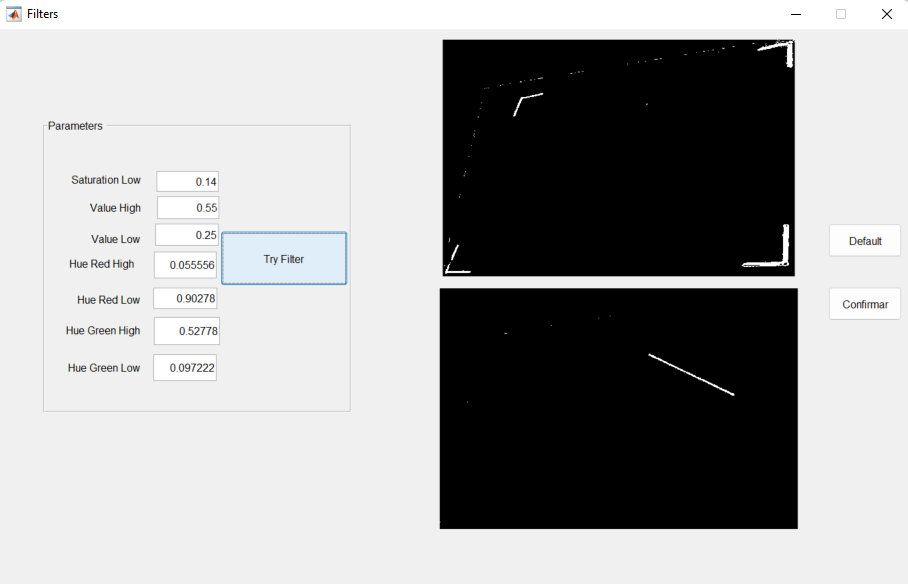
\includegraphics[width=\linewidth]{filtros}
	\caption{Pantalla de configuración de filtros.}	
	\label{fig:filtros}
\end{figure}

\Section{Errores comunes}

\begin{itemize}
	\item El programa debe ser corrido desde main.m y no desde otro archivo.
	\item No aparece le manipulador al cargar la imagen:
Existen veces que el Matlab y el Robotics Toolbox no interaccionan correctamente y no carga el manipulador, para resolver este problema basta con reiniciar Matlab hasta que funcione o reinstalar el toolbox.
	\item El mismo gráfico se muestra en mas de un cuadro:\\
Sucede cuando se mueve el manipulador y se rota otra imagen, esto se debe a que el toolbox grafica en el cuadro que esta siendo seleccionado, y no deja que se configure, por lo que no debe tocarse otro cuadro mientras se mueve el manipulador.
	\item Cuando se filtra una imagen aparece el error ``Assignment not supported because the result method `umin'\, is a temporary value'':\\
Error propio del toolbox que a veces no reconoce bien parámetros poropios. Similar a cuando no carga el manipulador.
\end{itemize}

\end{document}